\chapter{Implementacija i korisničko sučelje}
		
		
		\section{Korištene tehnologije i alati}
		
			
			  U izradi projekta većina digitalne komunikacije ostvarena je preko platforme
			  \textbf{WhatsApp} (\textit{https://web.whatsapp.com/} ).

			  Korištene su sljedeće tehnologije i alati:

			  \begin{packed_item}

				\item \textbf{Springboot}
					\begin{packed_item}
						\item open source radni okvir za kreaciju mikro-servisa, idealan za potrebe projekta
						\item u njemu je izrađen backend dio projekta 
						\item \textit{https://spring.io/projects/spring-boot}
					\end{packed_item}

				\item \textbf{React}
				\begin{packed_item}
					\item JavaScript biblioteka za izgradnju korisničkih sučelja 
					\item korišten za izradu čitavog frontenda dijela aplikacije s kojim korisnik dolazi u interakciju 
					\item provjerava ispravnost podataka unesenih u obrasce 
					\item \textit{ https://www.reactjs.org/}
				\end{packed_item}

				\item \textbf{PostgreSQL }
				\begin{packed_item}
					\item jezik u kojem je napravljena baza podataka  
					\item besplatan i open source sustav za upravljanje relacijskim bazama podataka s naglaskom na mogućnosti proširivanja  
					\item \textit{ https://www.postgresql.org/}
				\end{packed_item}
				
				\item \textbf{pgAdmin}
				\begin{packed_item}
					\item za upravljanje bazom podataka neovisno o backendu 
					\item \textit{ https://www.pgadmin.org/}
				\end{packed_item}

				\item \textbf{IntelliJ }
				\begin{packed_item}
					\item  IDE za javu u kojem je kodiran backend dio projekta 
					\item \textit{ https://www.jetbrains.com/idea/}
				\end{packed_item}

				\item \textbf{Visual Studio Code}
				\begin{packed_item}
					\item  uređivač izvornog koda za razne programske jezike
					\item  korišten za kodiranje frontend dijela projekta i projektne dokumentacije
					\item \textit{ https://code.visualstudio.com/}
				\end{packed_item}

				\item \textbf{Astah UML }
				\begin{packed_item}
					\item program za uređivanje svih vrsta UML dijagrama
					\item svi dijagrami u ovom dokumentu izrađeni su u Astahu 
					\item \textit{https://astah.net/products/astah-uml/}
				\end{packed_item}

				\item \textbf{GitHub }
				\begin{packed_item}
					\item  stranica za funkcionalno zajedničko stvaranje i uređivanje grupnog projekta 
					\item \textit{https://github.com/}
				\end{packed_item}

				\item \textbf{Latex}
				\begin{packed_item}
					\item programski jezik za pisanje strukturiranih tekstova, često korišten za stvaranje profesionalnih dokumenata
					\item koristi markup jezik koji prevodi u formatirane dokumente
					\item korišten za dokumentiranje projekta
					\item \textit{https://www.latex-project.org/}
				\end{packed_item}
				
				\item \textbf{Render}
				\begin{packed_item}
					\item cloud platforma za izradu i besplatno hostanje web-aplikacija i stranica
					\item korišten za puštanje \textit{backenda} i \textit{frontenda} u pogon i hostanje baze podataka
					\item \textit{https://www.render.com/}
				\end{packed_item}

				\item \textbf{Render}
				\begin{packed_item}
					\item cloud platforma za izradu i besplatno hostanje web-aplikacija i stranica
					\item korišten za puštanje \textit{backenda} i \textit{frontenda} u pogon i hostanje baze podataka
					\item \textit{https://www.render.com/}
				\end{packed_item}

				\item \textbf{Selenium}
				\begin{packed_item}
					\item program za automatizaciju web aplikacija u svrhe testiranja
					\item korišten za ispitivanje
					\item \textit{https://www.selenium.dev}
				\end{packed_item}
			\end{packed_item}
			

			 \eject 
		
	
		\section{Ispitivanje programskog rješenja}
			
			\subsection{Ispitivanje komponenti}
			Napravljen je java file za provođenje testova BackendApplicationTests.java sa JUnit testovima koji provjeravaju:

			\begin{packed_item}
					\item vraća li grešku funkcija za dohvaćanje korisnika s nepostojećim korisničkim imenom - testGetUserByUsernameThatDoesNotExist
					\item vraća li funkcija pravog korisnika za dohvaćanje korisnika s postojećim korisničkim imenom -  testGetUserByUsernameThatExists
					\item hoće li funkcija baciti grešku ako je uneseno ime nepostojeće postaje – testStationAlreadyHasManagerNonExistentStation
					\item hoće li funkcija za nepostojeći ID vozila baciti gresku – testFindVehicleByNonexistentId
					\item hoće li funkcija za dobro ime, ali lošu lozinku vratiti False – testLoginInvalidPassword
					\item hoće li funkcija vratiti True ako stanica već ima dodijeljenog voditelja - testStationAlreadyHasManager
				\end{packed_item}
			
			
			\begin{figure}[H]
				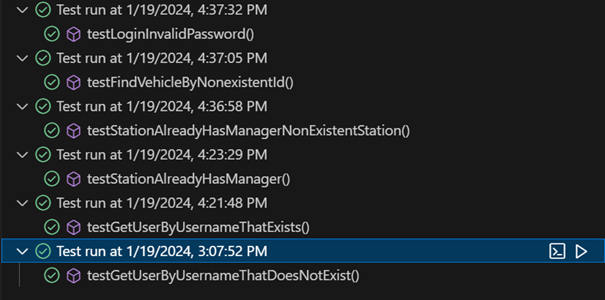
\includegraphics[scale=0.85]{slike/Zadovoljeni testovi.png}
				\centering
				\caption{Zadovoljeni testovi}
				\label{fig:Zadovoljeni testovi}
			\end{figure}

			\begin{figure}[H]
				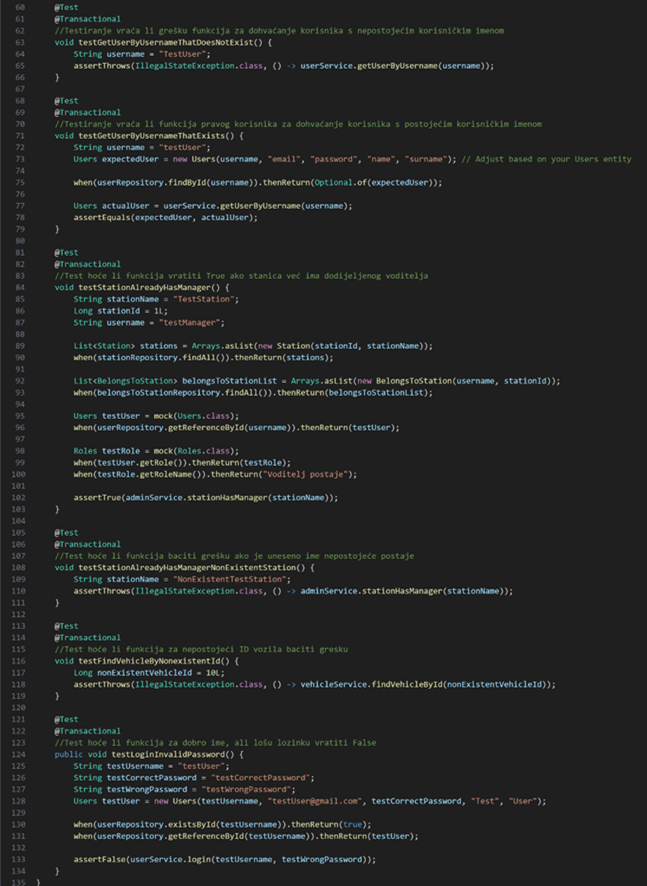
\includegraphics[scale=1]{slike/BackendApplicationTests.png}
				\centering
				\caption{Kod BackendApplicationTests.java}
				\label{fig:BackendApplicationTests}
			\end{figure}


			%%%%%%%%%%%%%%%%%%%%%%%%%%%%%%%%%%%%%%%%%%%%%%%%%%%%
			\subsection{Ispitivanje sustava}

			\textbf{Testovi sustava}
			Provedeni su testovi administratorove mogućnosti uređivanja podataka 
			korisnika, mogućnost voditelja postaje da na svoju postaju doda 
			tragače koji nisu dodijeljeni nijednoj drugoj postaji, mogućnost 
			istraživača da prouči informacije pojedinim jedinkama životinja 
			te mogućnost da mu se na karti prikazuju mjesta gdje se pojedine 
			vrste životinja kreću.
	
			\textit{\textbf{Mijenjanje podataka o korisnicima}}
			\newline
			Za test mijenjanja podataka o korisnicima koriste se ulazni podaci 
			„admin“ za korisničko ime te „password“ za lozinku. 

			

			Pritiskom na gumb „Prijava“ prikazuje nam se početna stranica za 
			administratora. Odaberemo opciju „Pregled korisnika“ te 
			na popisu korisnika odaberemo korisnika s korisničkim imenom 
			„tragac10“. Prikazuje nam se stranica sa svim podacima o navedenom 
			korisniku te opcije „Izbriši korisnika“ i „Promjeni podatke“. 
			Odaberemo opciju „Promijeni podatke“ te nakon što nam se otvori 
			forma za mijenjanje podataka, odaberemo polje ispod teksta „Email:“. 
			Kao novu adresu unesemo tragac15@gmail.hr te pritisnemo na tipku 
			„Spremi promjene“. Nakon toga ponovno nam se otvara stranica s 
			opcijama „Pregled korisnika“ i „Pregled zahtjeva“. Ponovno 
			odaberemo opciju „Pregled korisnika“ te pronađemo korisnika s 
			korisničkim imenom „tragač10“. Nakon što pritisnemo na tog korisnika,
			 otvara nam se stranica s njegovim podacima gdje možemo vidjeti 
			 njegovu izmijenjenu email adresu.

\begin{figure}[H]
				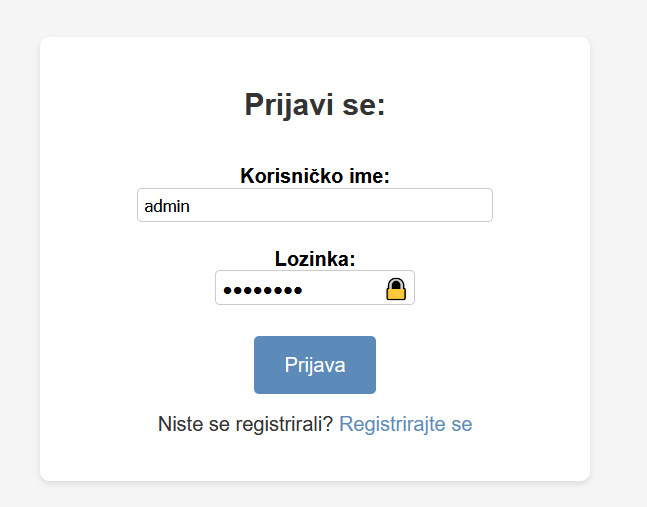
\includegraphics[scale=0.6]{slike/test11.png}
				\centering
				\caption{Mijenjanje podataka o korisnicima korak 1}
				\label{fig:Mijenjanje podataka o korisnicima korak 1}
			\end{figure}

			\begin{figure}[H]
				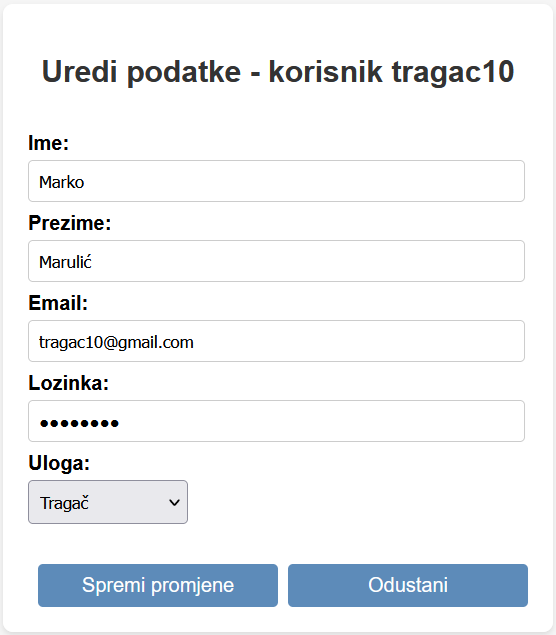
\includegraphics[scale=0.6]{slike/test12.png}
				\centering
				\caption{Mijenjanje podataka o korisnicima korak 2}
				\label{fig:Mijenjanje podataka o korisnicima korak 2}
			\end{figure}

			\begin{figure}[H]
				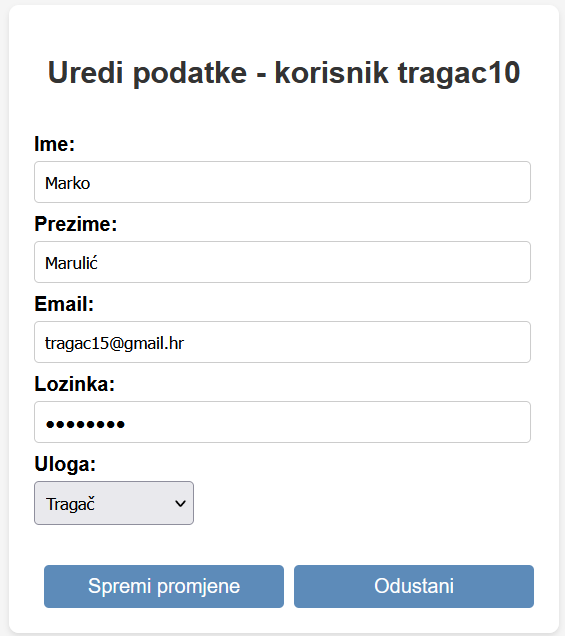
\includegraphics[scale=0.6]{slike/test13.png}
				\centering
				\caption{Mijenjanje podataka o korisnicima korak 3}
				\label{fig:Mijenjanje podataka o korisnicima korak 3}
			\end{figure}

			\begin{figure}[H]
				
\includegraphics[scale=0.7]{slike/test14.png}
				\centering
				\caption{Mijenjanje podataka o korisnicima korak 4}
				\label{fig:Mijenjanje podataka o korisnicima korak 4}
			\end{figure}



			\textit{\textbf{Dodavanje tragača na postaju}}
			\newline
			Za test dodavanja tragača na postaju u ulozi voditelja postaje koriste se ulazni 
			podaci „waiting“ za korisničko ime te „password“ za lozinku. Pritiskom na gumb 
			„Prijava“ prikazuje nam se početna stranica za korisnike u ulozi voditelja postaje. 
			Pojavljuje nam se tekst s postajom kojom upravlja prijavljeni voditelj te pet opcija 
			za odabir. Nude se opcije „Pregled svih tragača“, „Pregled svojih tragača“, „Pregled 
			akcija“, „Pregled zahtjeva“ te „Moj profil“ (u gornjem desnom kutu). Odaberemo opciju 
			„Pregled svih tragača“, nakon čega nam se otvara prozor s tekstom „Pregled svih tragača“ 
			te ispod njega popis svih tragača koji trenutno nemaju dodijeljenu postaju. 
			Pritiskom na kućicu ispod pripadajućeg tragača, nudi nam se šest različitih 
			vozila za dodjeljivanje kao sposobnosti odabranom tragaču. Odaberemo tragača s 
			imenom „test“ te prezimenom „tragac“. Nakon toga mu kao prijevozna sredstva dodijelimo 
			mogućnosti „pješke“ te „dronom“. Pritiskom na gumb „Potvrdi“ potvrđujemo svoj odabir. 
			Nakon što smo potvrdili svoj odabir, ponovno se otvara početna stranica korisnika u ulozi 
			voditelja postaje. Ovaj put odaberemo opciju „Pregled svojih tragača“, nakon čega nam se  
			otvara prozor sa tekstom „Lista svojih tragača“ te ispod njega popis svih tragača 
			dodijeljenih postaji, s njihovim osnovnim korisničkim podacima. Možemo vidjeti da se 
			sada i na popisu nalazi tragač s imenom „test“ i prezimenom „tragac“.



			\begin{figure}[H]
				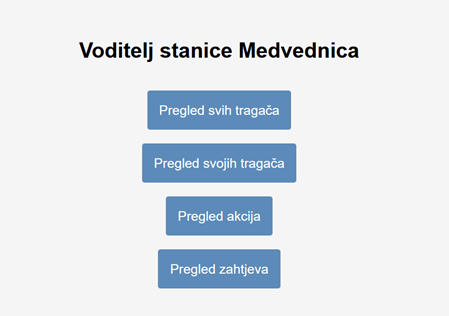
\includegraphics[scale=0.8]{slike/Dodavanje tragača na postaju korak 1.png}
				\centering
				\caption{Dodavanje tragača na postaju korak 1}
				\label{fig:Dodavanje tragača na postaju korak 1}
			\end{figure}

			\begin{figure}[H]
				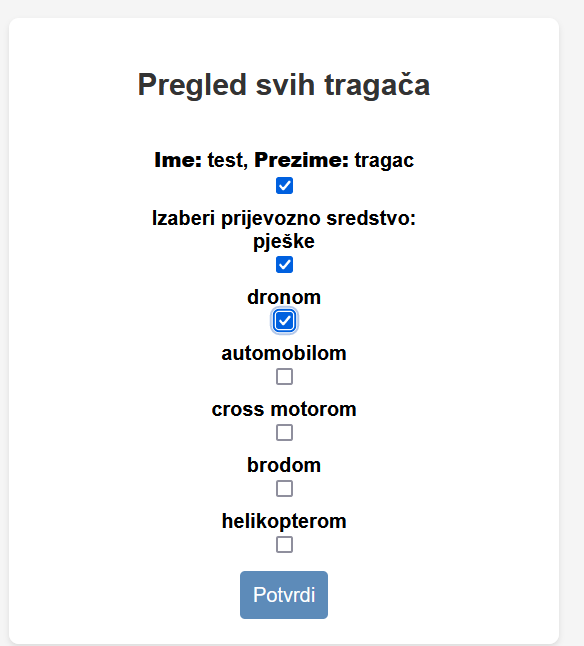
\includegraphics[scale=0.62]{slike/Dodavanje tragača na postaju korak 2.png}
				\centering
				\caption{Dodavanje tragača na postaju korak 2}
				\label{fig:Dodavanje tragača na postaju korak 2}
			\end{figure}

			\begin{figure}[H]
				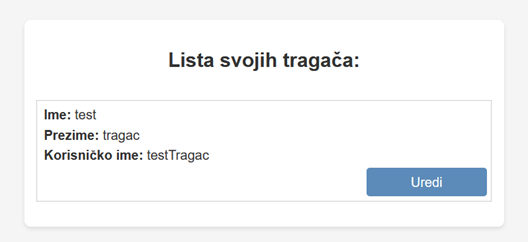
\includegraphics[scale=0.85]{slike/Dodavanje tragača na postaju korak 3.png}
				\centering
				\caption{Dodavanje tragača na postaju korak 3}
				\label{fig:Dodavanje tragača na postaju korak 3}
			\end{figure}


			\textit{\textbf{Pregled informacija o životinjama}}
			\newline

			Za test pregleda informacija o životinjama u ulozi istraživača koriste se ulazni 
			podaci „istrazivacXmouse“ za korisničko ime te „lozinka1“ za lozinku. Pritiskom 
			na gumb „Prijava“ prikazuje nam se početna stranica za korisnike u ulozi 
			istraživača. Za odabir nam se nude opcije „Popis akcija“, „Karta – životinje“,
			 „O životinjama“ te „Moj profil“ (u gornjem desnom kutu). Odaberemo opciju 
			 „O životinjama“. Otvara nam se izbornik s različitim vrstama životinja. 
			 Odaberemo opciju „Sivi vuk“ te nakon što nam se prikaže prozor s popisom 
			 jedinki te vrste, odaberemo opciju „Sivi vuk, id: 7“. Otvara nam se prozor u 
			 kojemu možemo vidjeti sliku pripadajuće vrste, njen latinski naziv, detaljan opis 
			 vrste te komentare ostalih korisnika vezanih uz navedenu jedinku. Dodatno, nudi 
			 nam se mogućnost brisanja te pisanja vlastitih komentara.



			\begin{figure}[H]
				\includegraphics[scale=0.6]{slike/Pregled informacija o životinjama korak 1.png}
				\centering
				\caption{Pregled informacija o životinjama korak 1}
				\label{fig:Pregled informacija o životinjama korak 1}
			\end{figure}

			\begin{figure}[H]
				\includegraphics[scale=0.55]{slike/Pregled informacija o životinjama korak 2.png}
				\centering
				\caption{Pregled informacija o životinjama korak 2}
				\label{fig:Pregled informacija o životinjama korak 2}
			\end{figure}

			\begin{figure}[H]
				\includegraphics[scale=0.6]{slike/Pregled informacija o životinjama korak 3.png}
				\centering
				\caption{Pregled informacija o životinjama korak 3}
				\label{fig:Pregled informacija o životinjama korak 3}
			\end{figure}


			\textit{\textbf{Pregled staništa vrste na karti}}
			\newline
			Za test pregleda staništa pojedine vrste životinja na karti u ulozi istraživača 
			koriste se ulazni podaci „ju54164“ za korisničko ime te „lozinka1“ za lozinku. 
			Pritiskom na gumb „Prijava“ prikazuje nam se početna stranica za korisnike u 
			ulozi istraživača. Za odabir nam se nude opcije „Popis akcija“, 
			„Karta – životinje“, „O životinjama“ te „Moj profil“ (u gornjem desnom kutu). 
			Odaberemo opciju „Karta – životinje“. Otvara nam se prozor u čijem se središtu 
			nalazi karta, a u gornjem lijevom kutu dvije opcije za prikaz na karti, 
			„Po vrsti“ te „Po jedinci“. Odaberemo opciju „Po vrsti“, nakon čega nam se 
			ispod pojavljuje popis svih mogućih vrsta. Pritiskom na gumb „Sivi sokol“, 
			na karti nam se pojavljuje heatmap svih povijesnih lokacija jedinki koje 
			pripadaju toj vrsti. 


			\begin{figure}[H]
				\includegraphics[scale=0.75]{slike/Pregled staništa vrste na karti korak 1.png}
				\centering
				\caption{Pregled staništa vrste na karti korak 1}
				\label{fig:Pregled staništa vrste na karti korak 1}
			\end{figure}

			\begin{figure}[H]
				\includegraphics[scale=1]{slike/Pregled staništa vrste na karti korak 2.png}
				\centering
				\caption{Pregled staništa vrste na karti korak 2}
				\label{fig:Pregled staništa vrste na karti korak 2}
			\end{figure}

			\begin{figure}[H]
				\includegraphics[scale=1]{slike/Pregled staništa vrste na karti korak 3.png}
				\centering
				\caption{Pregled staništa vrste na karti korak 3}
				\label{fig:Pregled staništa vrste na karti korak 3}
			\end{figure}




		%%%%%%%%%%%%%%%%%%%%%%%%%%%%%%%%%%%%%%%%%%%%%%%%%%%%%%%%%%%%%%%%%%%%%%%%%%%%%%%%%%%%%%%%%%%%%%%%%%%%%%%
		\section{Dijagram razmještaja}

		UML-dijagram razmještaja je vrsta strukturnog UML-dijagrama 
		koji prikazuje fizičku arhitekturu i konfiguraciju 
		razmještaja programskog sustava. Dijagram razmještaja koristan je 
		za vizualizaciju kako su komponente sustava raspoređene na fizičkim 
		računalima i kako međusobno komuniciraju.
		Na poslužiteljskom računalu se 
		nalaze web poslužitelj i poslužitelj baze podataka. Korisnici preko svog računala koriste web
		preglednik kako bi pristupili web aplikaciji. Sustav je baziran na arhitekturi 
		”klijent - poslužitelj”, a komunikacija između računala korisnika, 
		koji može biti tragač, istraživač, voditelj postaje ili administrator, i poslužitelja se 
		odvija preko HTTP veze, što je tipičan način komunikacije u web okolinama.

		\begin{figure}[H]
			\includegraphics[scale=0.7]{slike/dijagram razmještaja.png}
			\centering
			\caption{Dijagram razmještaja}
			\label{fig:dijagram razmještaja}
		\end{figure}
			\eject 
	%%%%%%%%%%%%%%%%%%%%%%%%%%%%%%%%%%%%%%%%%%%%%%%%%%%%%%%%%%%%%%%%%%%%%%%%%%%%%%%%%%%%%%%%%%%%%%%%%%%%%%%%%%%%%%%%%%%%%%%%%
	%%%%%%%%%%%%%%%%%%%%%%%%%%%%%%%%%%%%%%%%%%%%%%%%%%%%%%%%%%%%%%%%%%%%%%%%%%%%%%%%%%%%%%%%%%%%%%%%%%%%%%%%%%%%%%%%%%%%%%%%%
	%%%%%%%%%%%%%%%%%%%%%%%%%%%%%%%%%%%%%%%%%%%%%%%%%%%%%%%%%%%%%%%%%%%%%%%%%%%%%%%%%%%%%%%%%%%%%%%%%%%%%%%%%%%%%%%%%%%%%%%%%

		\section{Upute za puštanje u pogon}
		
			Puštanje web aplikacije u pogon sastoji se od tri segmenta:

			\begin{packed_item}
				\item Stvaranje baze podataka
				\item Puštanje \textit{backend-a} u pogon
				\item Puštanje \textit{frontend-a} u pogon
			\end{packed_item}

			\subsubsection{Stvaranje baze podataka}

			Baza podataka besplatno je spremljena na web-oblaku render.com. 
			Ona se postavlja i osposobljava sljedećim koracima:

			\begin{packed_enum}
				\item Stvaranje nove baze
				
				\begin{packed_item}
					\item Potrebno je (nakon registracije na render.com) odabrati opciju New te na padajućem izborniku PostgreSQL
					\item Pojavljuje se izbornik koji ispunjavamo kao na slici \ref{fig:postavljanje baze1}
					\item Biramo \textit{Create Database}
				\end{packed_item}

			\begin{figure}[H]
				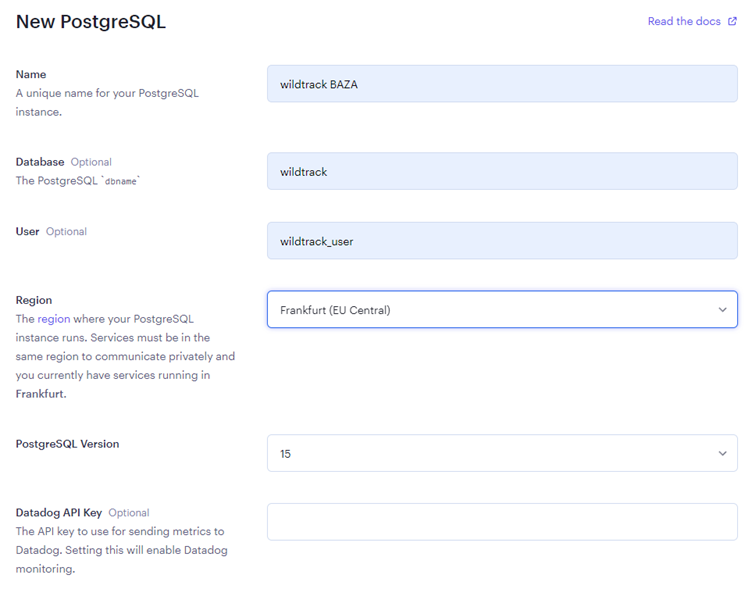
\includegraphics[scale=1]{slike/postavljanje baze1.png}
				\centering
				\caption{Stvaranje nove PostgreSQL baze}
				\label{fig:postavljanje baze1}
			\end{figure}

			 \item Dohvat podataka za spajanje
			 \begin{packed_item}
				\item Odabiremo \textit{Dashboard -  wildtrack BAZA -  Info}
				\item Spuštamo stranicu do izbora \textit{Connections} sa informacijama potrebnim za spajanje na bazu (slika \ref{fig:postavljanje baze2}).
			\end{packed_item}

			\begin{figure}[H]
				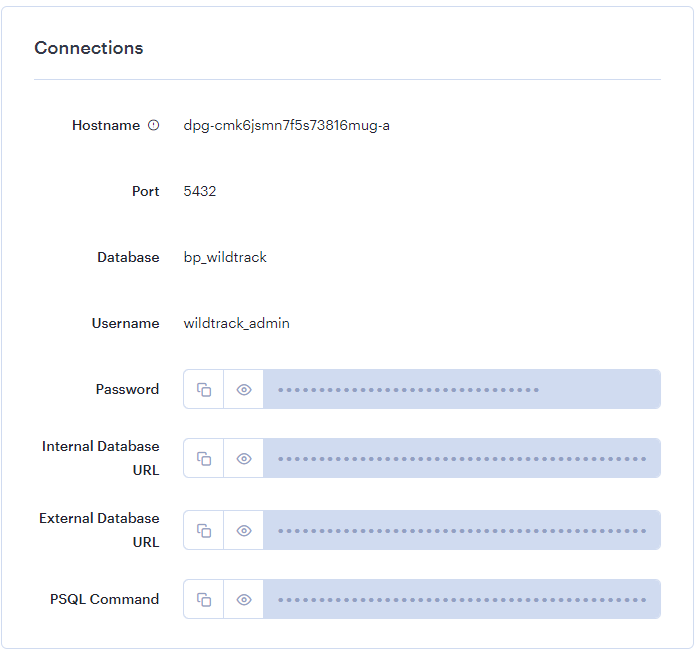
\includegraphics[scale=1]{slike/postavljanje baze2.png}
				\centering
				\caption{Dohvat podataka za spajanje baze}
				\label{fig:postavljanje baze2}
			\end{figure}

			\item Spajanje putem pgAdmina
			\begin{packed_item}
				\item Odabiremo \textit{Object - Create - Server}
				\item Na kartici \textit{General} unosimo ime servera kojeg otvaramo u pgAdminu
				\item Na kartici \textit{Connection} unosimo podatke kao na slici \ref{fig:postavljanje baze3} i spremamo ih sa \textit{Save}
			\end{packed_item}

			\begin{figure}[H]
				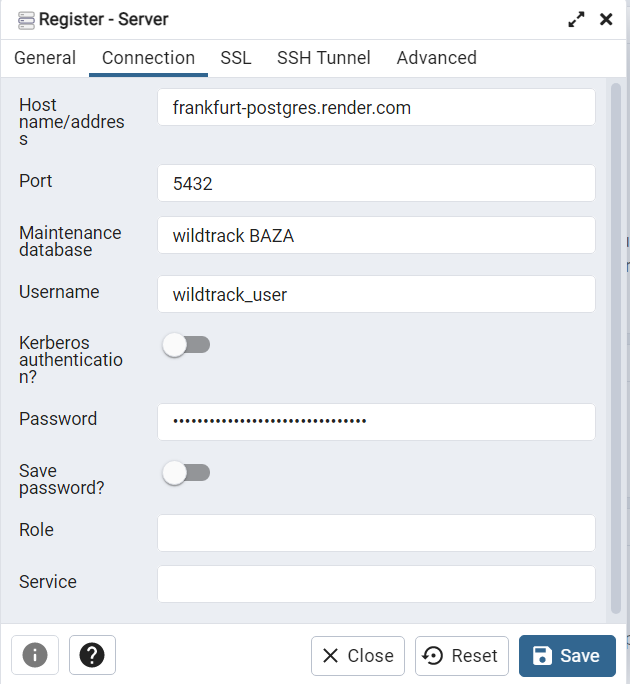
\includegraphics[scale=1]{slike/postavljanje baze3.png}
				\centering
				\caption{Unos podataka za spajanje baze}
				\label{fig:postavljanje baze3}
			\end{figure}

			\item Spajanje iz \textit{backenda}
			\begin{packed_item}
				\item U \textit{src/main/resources/application.properties} upisujemo naredbe sa slike \ref{fig:postavljanje baze4}
			\end{packed_item}
			
			\begin{figure}[H]
				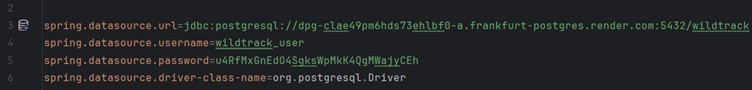
\includegraphics[scale=1]{slike/postavljanje baze4.png}
				\centering
				\caption{Spajanje baze iz \textit{backenda}}
				\label{fig:postavljanje baze4}
			\end{figure}


			\end{packed_enum}

			\subsubsection{Puštanje backenda u pogon}

			Backend dio projekta također koristi render.com za puštanje u pogon. Preduvjeti za to su:
			\begin{packed_item}
				\item Dodavanje Dockerfile-a prikazanog na slici \ref{fig:dockerfile}
				\item povezivanje s GitHub-om na renderu
			\end{packed_item}

			\begin{figure}[H]
				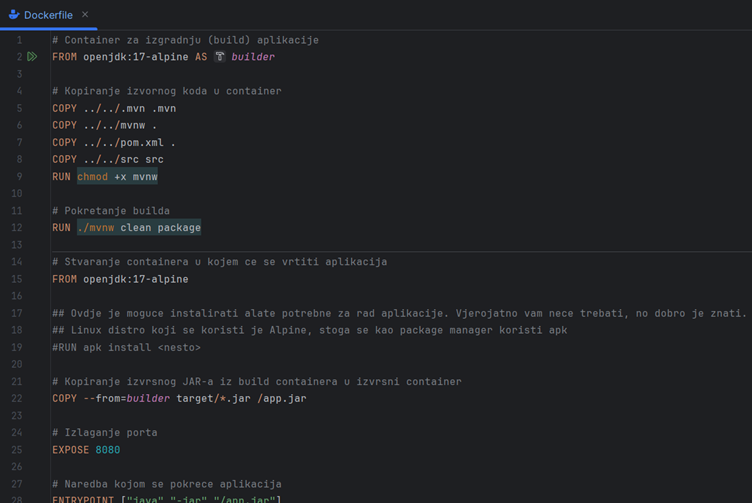
\includegraphics[scale=1]{slike/dockerfile.png}
				\centering
				\caption{Potrebni Dockerfile}
				\label{fig:dockerfile}
			\end{figure}

			Stvaranje backenda postižemo na sljedeći način:
			\begin{packed_item}
				\item Odabiremo na renderu \textit{New - Web Service}
				\item Odabiremo željeni GitHub repozitorij
				\item Unosimo tražene podatke i potvrđujemo s \textit{Create Web Service}
			\end{packed_item}

			\subsubsection{Puštanje frontenda u pogon}

			Frontend dio projekta također koristi render.com za puštanje u pogon. Preduvjeti za to su:
			
			\begin{packed_item}
				\item U IzvorniKod/package.json dodajemo dependency-e (primarno http-proxy-middleware, dotenv, express) kao na slici \ref{fig:frontendDeploy1}
				
			\begin{figure}[H]
				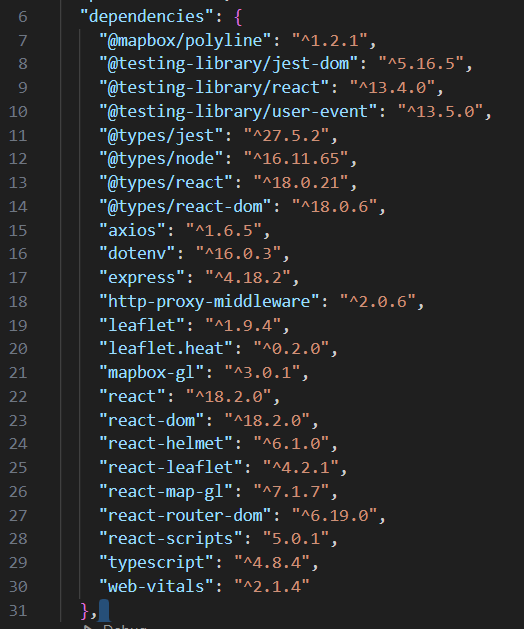
\includegraphics[scale=1]{slike/frontendDeploy1.png}
				\centering
				\caption{Dio koda package.json \textit{dependency}}
				\label{fig:frontendDeploy1}
			\end{figure}
			
				\item U IzvorniKod/package.json dodajemo kod kao na slici \ref{fig:frontendDeploy2} zbog funkcionalnosti Node-a
				
			\begin{figure}[H]
				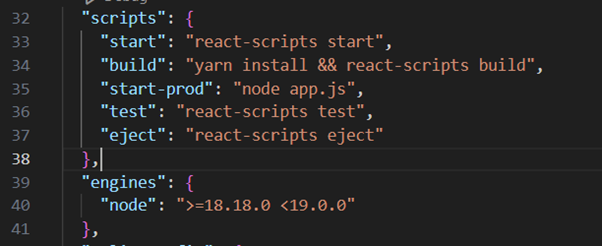
\includegraphics[scale=1]{slike/frontendDeploy2.png}
				\centering
				\caption{Dio koda package.json za funkcionalnost\textit{Node-a}}
				\label{fig:frontendDeploy2}
			\end{figure}
			
				\item Dodajemo /src/setupProxy.js koji služi kao proxy server za lokalni development (preusmjerava api pozive na localhost:8080)
				\item Dodajemo app.js, u kojem se nalazi express server za produkcijski proxy i posluživanje \textit{frontenda} (slika \ref{fig:frontendDeploy3})
			
			\begin{figure}[H]
				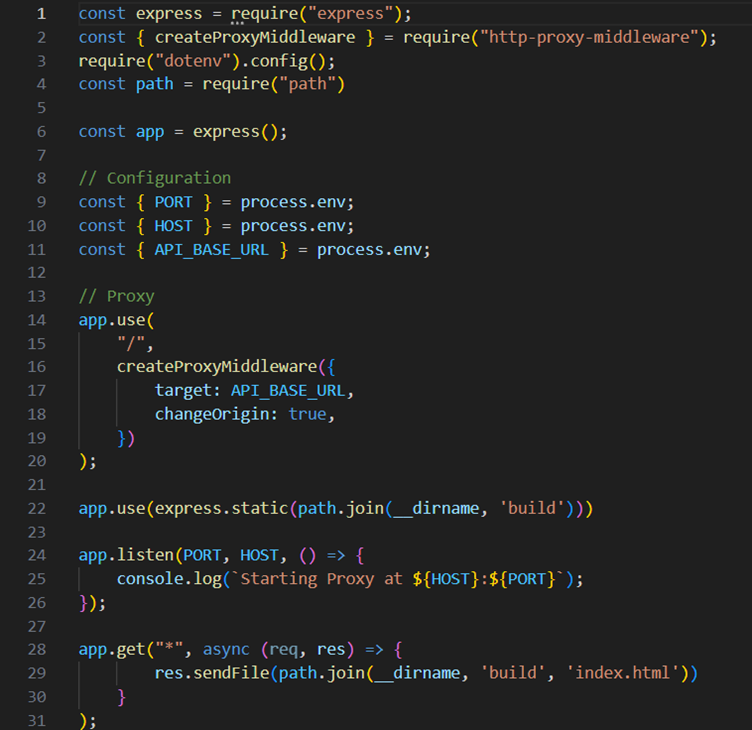
\includegraphics[scale=1]{slike/frontendDeploy3.png}
				\centering
				\caption{Kod datoteke app.js}
				\label{fig:frontendDeploy3}
			\end{figure}

			Stvaranje frontenda postižemo na sljedeći način:
			\begin{packed_item}
				\item Odabiremo na renderu \textit{New - Web Service}
				\item Odabiremo željeni GitHub repozitorij
				\item Unosimo tražene podatke (slika \ref{fig:frontendDeploy4})
				\item Potvrđujemo s \textit{Create Web Service}
			\end{packed_item}

			\begin{figure}[H]
				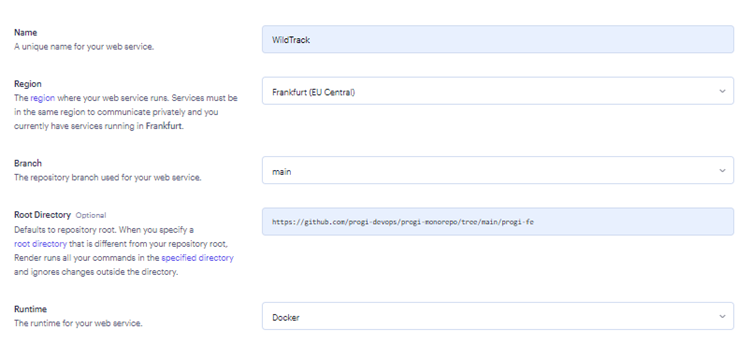
\includegraphics[scale=1]{slike/frontendDeploy4.png}
				\centering
				\caption{Spajanje \textit{frontenda}}
				\label{fig:frontendDeploy4}
			\end{figure}

		
		\end{packed_item}
			
			

			

			



			\eject 